\chapter[Marco Teórico]{\label{ch:marco-teorico}Marco Teórico}

\section{Sistemas Multi-core y OpenMP}

En este capitulo se describen los conocimientos basicos sobre programación multi-nucleos, programación en coprocesadores tales como progración en Intel Xeon Phi, programación en GPU y trabajos relacionados que dan base a esta tesis.\\
Actualmente las arquitecturas de los dispositivos personales estan diseñadas con multiprocesadores o coprocesadores, desde un equipo de bolsillo como un celular (Smartphone) hasta un computador personal (notebook), esto quiere decir que los dispositivos cuentan con varios nucleos en una sola CPU (Unidad central de procesamiento) en el caso de multiprocesadores y con más de una CPU en el caso de un Coprocesador.\\

\subsection{Threads}
Existen varias bibliotecas que permiten la programación en multi-hilos, con esto somos capaces de ejecutar hilos en paralelo, ejecutándose en un núcleo diferente.\\
Exiten diferentes modelos y estandares que permiten la programación de múltiples hilos, tales como Pthreads \cite{libroPthreads}, TBB \cite{libroTBB} u OpenMP \cite{libroOpenMP}, en particular en esta tesis se selecciono el uso de la biblioteca OpenMP que fue desarrollada en 1997. Además es importante mencionar el hecho de que actualmente los compiladores en esta linea son bastante robustos, como tambien el hecho de que el equipo que gestiona OpenMP esta conformado por diferentes compañias (AMD, Intel, Sun Mycrosystem y otros) y no siendo gestionada por una sola, esto nos proporciona confianza.\\

\section{Coprocesadores}

Un Coprocesador es utilizado para desligar funciones de la CPU, en esta linea existen desde coprocesadores matematicos hasta coprocesadores graficos, estos poseen caracteristicas y espeficiaciones a ciertos tipos de operaciones, por ejemplo un coprocesador matematico solo esta desarrollado para revolver problemas aritmeticos o afines al área esto quiere decir que pueden realizar operaciones matematicas a una velocidad mayor que el procesador principal (CPU), a su vez un coprocesador gráfico esta diseñado en otra área. Estos proporcionan al hardware una acelaración en la operación solo cuando se ejecuta una tárea o software que se haya diseñado para aprovechar el coprocesador, las intrucciones para un coprocesador son diferentes que las intrucciones de una CPU de modo que existe un programa que detecta la existencia de un coprocesador y entonces se ejecutan las intrucciones escritas explicitamente para aquel coprocesador, por tanto existen diferentes lineas de coprocesadores en el mercado pero en esta tesis solo consideramos Intel Xeon Phi y GPU NVIDIA.

\subsection{Intel Xeon Phi}

El coprocesador Intel Xeon Phi \cite{xeonphi1} \cite{wange2014} \cite{xeonphila} consta de hasta 72 conectados en un anillo bidireccional de alto rendimiento en el chip. El coprocesador ejecuta un sistema operativo linux y es compatible con todas las principales herramientas de desarrollo de Intel como C / C ++, Fortran, MPI y OpenMP. El coprocesador se conecta a un procesador Intel Xeon (el host) a través del bus PCI Express (PCIe). Las propiedades más importantes de la arquitectura MIC se muestran en figura \ref{estructuraxeon}.\\

\textbf{Core:} El núcleo de la intel Xeon phi (Scalar Unit en la figura \ref{estructuraxeon}) es una arquitectura de orden (basada en la familia de procesadores Intel Pentium),Implementa instrucciones de recuperación y decodificación para 4 hilos (hardware) por núcleo. Las intrucciones vectoriales que posee el coprocesador Intel Xeon Phi, utiliza una unidad de punto flotante (VPU) dedicada, con un ancho de 512-bit, la que está disponible en cada núcleo. Un núcleo puede ejecutar dos intrucciones por ciclo de reloj, una en U-pipe y otra en V-pipe (no todos los tipos de instrucciones pueden ser ejecutadas por el V-pipe). Cada núcleo compone una interconexión en anillo mediante la CRI (Core Ring Interface).\\

\textbf{Vector Processing Unit (VPU):} La VPU incluye la EMU (Extended Math Unit), y es capaz de realizar 16
operaciones en punto flotante con precisión simple por ciclo, 16 operaciones de enteros de 32-bit por ciclo u
8 operaciones en punto flotante con precisión doble por ciclo.\\

\textbf{L1 Cache:} Tiene una caché L1 de 32KB para instrucciones y de 32KB para datos, asociativa de 8-vías,
con tamaño de línea de caché de 64 bytes. Tiene una latencia de cargado de 1 ciclo, que significa que un valor
entero cargado desde L1 puede ser usado en el siguiente ciclo por una instrucción entera (instrucciones vectoriales
tienen diferente latencia que las enteras).\\

\textbf{L2 Cache:} Cada núcleo posee 512KB de caché L2. Si ningún núcleo comparte algún dato o código, entonces el
tamaño total de la caché L2 es de 31 MB. Por otro lado, si todos los núcleos comparten exactamente el mismo
código y datos en perfecta sincronía, el tamaño total de la caché L2 sería solo de 512KB. Su latencia es de 11
ciclos de reloj.\\

\textbf{Ring:} Incluye interfaces y componentes, ring stops, ring turns, direccionamiento y control de flujo. Un coprocesador Xeon Phi tiene 2 de estos anillos, uno viajando en cada dirección (Figure \ref{estructuraxeon2}).\\

La Figura \ref{estructuraxeon2} ilustra una visión general de la arquitectura, donde se muestra como los núcleos están conectados con cachés coherentes mediante un anillo bidireccional de 115GB/sec. La figura también muestra una memoria GDDR5 con 16 canales de memoria, que alcanzan una velocidad de hasta 5.5GB/sec.

\begin{figure}[hbtp]
\centering
\label{estructuraxeon}
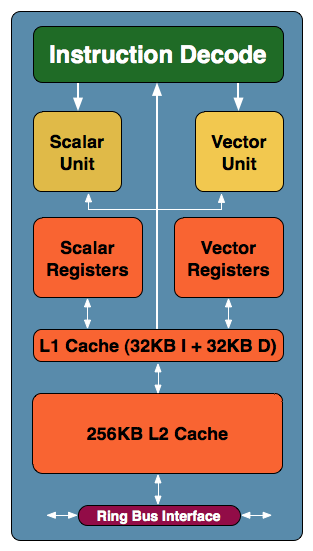
\includegraphics[scale=0.5]{fig/core.png}
\caption{Diagrama de una arquitectura MIC de un nucleo de un coprocesador Xeon Phi}
\end{figure}

\begin{figure}[hbtp]
\centering
\label{estructuraxeon2}
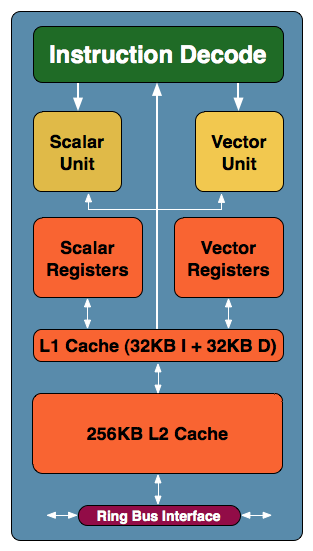
\includegraphics[scale=0.5]{fig/core.png}
\caption{Diagrama de una arquitectura MIC de un nucleo de un coprocesador Xeon Phi}
\end{figure}

\subsection{NVIDIA GPU}

Todas las implementaciones sobre GPU se realizaron usando el modelo de programación CUDA \cite{cuda} de NVIDIA. Este modelo hace una distinción entre el código ejecutado en la CPU (host) con su propia DRAM (host memory) y el ejecutado en GPU (device) sobre su DRAM (device memory). La GPU se representa como un coprocesador capaz de ejecutar funciones denominadas kernels, y provee extensiones para el lenguaje C que permiten alojar datos en la memoria de la GPU y transferir datos entre GPU y CPU. Por lo tanto, la GPU sólo puede ejecutar las funciones declaradas como kernels dentro del programa, y sólo puede usar variables alojadas en device memory, lo cual significa que todos los datos necesarios deberán ser movidos a esta memoria de forma previa a la ejecución La figura \ref{} muestra un esquema de la diferencia entre una CPU y una GPU. Esta última está especializada para cómputo intensivo, y por lo tanto más transistores están dedicados para el procesamiento de datos en vez de caching de datos y control de flujo. 

Esto implica que la GPU es capaz de realizar un mayor número de operaciones aritméticas en punto flotante que una CPU. El correcto aprovechamiento del sistema de memoria en la GPU es primordial. La figura \ref{} muestra un esquema del hardware de una GPU, la que consta de las siguientes características:


\begin{itemize}
	\item Una GPU está constituida por una serie de \textit{multiprocesadores}, donde cada uno de éstos cuenta con varios núcleos.

	\item Cada núcleo cuenta con sus propios registros y todos los núcleos del mismo multiprocesador comparten una \textit{shared memory}.

	\item \textbf{Shared memory} es una memoria que se encuentra próxima a los núcleos del multiprocesador, y por lo tanto es de muy baja latencia.
	
	\item Cada multiprocesador cuenta con un par de memorias caché compartidas por todos los núcleos, \textit{constant cache} y \textit{texture cache}.

	\item \textbf{Constant cache} es una caché de datos de la constant memory, que es una memoria de sólo lectura de reducido tamaño alojada en \textit{device memory}.

	\item \textbf{Texture cache} es una caché de la texture memory, que es una memoria optimizada para localidad espacial 2D, y está alojada en \textit{device memory}.

	\item \textbf{Device memory} es una memoria compartida por todos los multiprocesadores, y es de gran tamaño.

\end{itemize}



\subsection*{Organización y ejecución de threads}

Los threads son organizados en \textit{CUDA Blocks}, y cada uno de estos se ejecuta completamente en un único multiprocesador. Esto permite que todos los threads de un mismo CUDA Block compartan la misma \textit{shared memory}.
Un \textit{kernel} puede ser ejecutado por un número limitado de CUDA Blocks, y cada CUDA Block por un número acotado de threads. Sólo los threads que pertenecen al mismo CUDA Block pueden ser sincronizados. Es decir, hilos que pertenezcan a CUDA Blocks distintos sólo pueden ser sincronizados realizando un nuevo lanzamiento de kernel.

Para soportar la gran cantidad de threads en ejecución se emplea una arquitectura SIMT
(Single-Instruction, Multiple-Thread). La unidad de ejecución no es un thread, sino un \textit{warp}, que es un conjunto de threads, y un \textit{half-warp} corresponde a la primera o segunda mitad del conjunto de threads de un \textit{warp}. La forma en que un CUDA Block es dividido en \textit{warps} es siempre la misma, el primer conjunto de threads representan el primer \textit{warp}, el segundo conjunto consecutivo de threads el segundo \textit{warp} y así sucesivamente.

\subsection*{Reducción de lecturas a memoria}

Los accesos a memoria de un \textit{half-warp} a device memory son fusionados en una sola transacción de memoria si las direcciones accedidas caben en el mismo segmento de memoria. Por lo tanto, si los threads de un \textit{half-warp} acceden a \textit{n} diferentes segmentos, entonces se ejecutarán \textit{n} transacciones de memoria. Si es posible reducir el tamaño de la transacción, entonces se lee sólo la mitad de ésta.

\subsection*{Funciones atómicas}
Existe un grupo de funciones atómicas que realizan operaciones de tipo \textit{read-modify-write} sobre palabras de residentes en \textit{global memory o shared memory}. Estas funciones garantizan que serán realizadas completamente sin interferencia de los demás threads.
Cuando un thread ejecuta una función atómica, ésta bloquea el acceso a la dirección de memoria donde reside la palabra involucrada hasta que se complete la operación. Las funciones atómicas se dividen en funciones aritméticas y funciones a nivel de bits, a continuación se muestran algunas de las funciones aritméticas relevantes para el presente trabajo:

\begin{itemize}

	\item atomicAdd int atomicAdd(int *address, int val)

	Lee la palabra \textit{old} localizada en la dirección \textit{address} y escribe en la misma dirección el valor \textit{(old+val)}. El valor retornado es \textit{old}. Estas tres operaciones se realizan en una transacción atómica.

	\item atomicSub int atomicSub(int *address, int val)

	Lee la palabra \textit{old} localizada en la dirección \textit{address} y escribe en la misma dirección el valor \textit{(old-val)}. El valor retornado es \textit{old}. Estas tres operaciones se realizan en una transacción atómica.

	\item atomicMin int atomicMin(int *address, int val)

	Lee la palabra \textit{old} localizada en la dirección \textit{address} y escribe en la misma dirección el valor mínimo entre \textit{(old-val)}. El valor retornado es \textit{old}. Estas tres operaciones se realizan en una transacción atómica.

	 \item atomicMax int atomicMax(int *address, int val)

	Lee la palabra \textit{old} localizada en la dirección \textit{address} y escribe en la misma dirección el valor máximo entre \textit{(old-val)}. El valor retornado es \textit{old}. Estas tres operaciones se realizan en una transacción atómica.

\end{itemize}


\subsection*{Ejemplos}

\begin{figure}[hbtp]
\centering
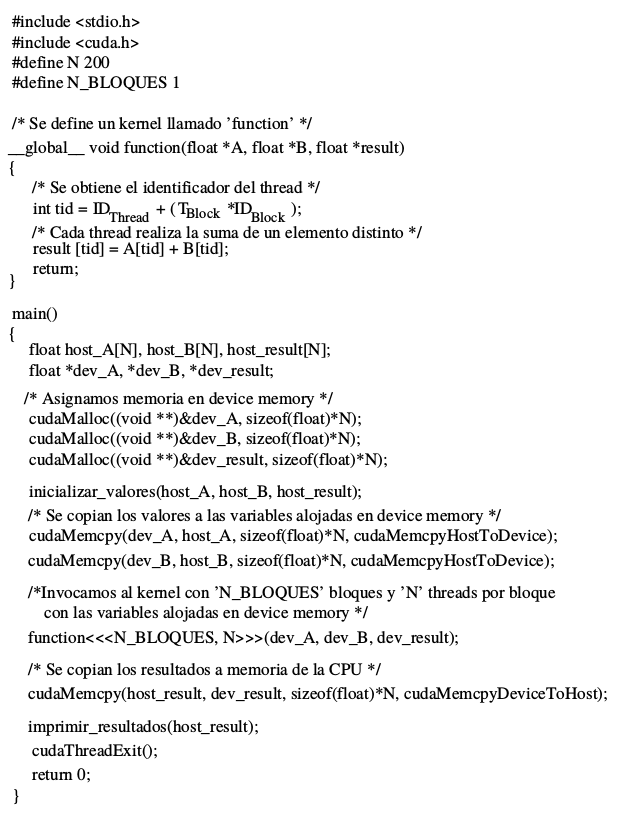
\includegraphics[scale=0.6]{fig/Ejemplo_gpu.png}
\caption{\label{ejemplo_gpu_suma}Ejemplo de suma de vectores con CUDA.}
\end{figure}

La figura \ref{ejemplo_gpu_suma} muestra un código que suma 2 vectores utilizando la GPU. Para esto primero se asigna memoria a los arreglos en device memory, luego se copian los valores necesarios a estas variables, y posteriormente se invoca al kernel con 1 CUDA Block (dado por la variable N\_BLOQUES ) y 200 threads por cada CUDA Block (dado por la variable N).

Cada thread obtiene su identificador (variable tid) usando variables predefinidas por la GPU, $ID_{Thread}$ (que retorna el ID del thread en el CUDA Block), $T_{Block}$ (que retorna la cantidad de threads de un CUDA Block) y $ID_{Block}$ (que retorna el identificador del CUDA Block). Cada thread realiza la suma del elemento tid-ésimo de ambos arreglos (dev\_A y dev\_B). Y ya una vez terminado el kernel se copia el arreglo resultado a la memoria de CPU para poder imprimir los resultados, pues no se puede invocar una función para imprimir dentro del kernel en la GPU utilizada.

Los threads de un warp siempre están sincronizados, es decir, ningún thread se puede adelantar a otro que pertenezca al mismo warp en la ejecución de instrucciones. Un ejemplo de esto lo muestra la figura \ref{cod_gpu_sync}, donde en el código \ref{cod_gpu_sync-a} se deben realizar instrucciones de sincronización para garantizar el correcto valor del arreglo result, mientras que el código \ref{cod_gpu_sync-b} es realizado solamente por los threads de un warp, y debido a esto no es necesario utilizar sincronización.


\begin{figure}
\begin{center}
\subfigure[Caption Subfigura 1]{
	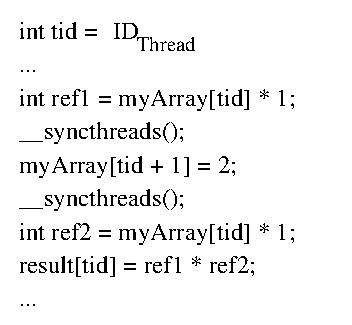
\includegraphics[width=5cm,height=4cm]{fig/cod_gpu_sync-a.eps}
    \label{cod_gpu_sync-a}
}~~~~~~~~~~~~
\subfigure[Caption Subfigura 2]{
	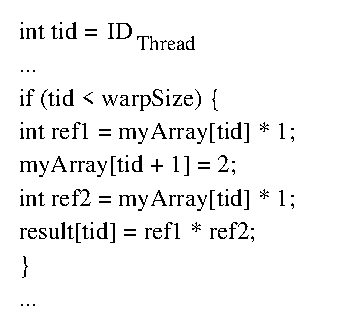
\includegraphics[width=5cm]{fig/cod_gpu_sync-b.eps}
    \label{cod_gpu_sync-b}
}
\caption{\label{cod_gpu_sync}Ejemplos para ilustrar la sincronizaci'on
de los threads de un \emph{warp}.}
\end{center}
\end{figure}